\documentclass[10pt, compress]{beamer}

\usetheme{m}

%\usepackage[T1]{fontenc}
\usepackage{booktabs}
\usepackage[scale=2]{ccicons}
\usepackage{minted}
\usepackage{color}
%\usepackage[usenames,dvipsnames]{xcolor}
\usepackage{tikz}
\usepackage{amsmath}
\usepackage{fixltx2e}
\usepackage{algpseudocode}

%\usetikzlibrary{external}
\usetikzlibrary{patterns}



%\tikzexternalize

\usemintedstyle{trac}

\MakeRobust{\Call}

\title{IF306 : Article Presentation}
\subtitle{On the k-coloring of intervals\\Martin C. Carlisle, Errol L. Lloyd}
\date{\today}
\author{Alexandre Honorat, Elouan Keryell-Even}
\institute{Enseirb-Matmeca}

\begin{document}

\maketitle

\section{Introduction}

\begin{frame}{Article topic}

\begin{block}{Problem}
\begin{itemize}
\item[$\bullet$]Coloring intervals
\item[$\bullet$]Different colors for intersecting intervals
\item[$\bullet$]$\mathnormal{P}$: Given the number of colors, trying to maximize the number of colored interval.
\end{itemize}
\end{block}
\begin{overlayarea}{\textwidth}{\textheight}

\only<2>{
\begin{block}{Example}
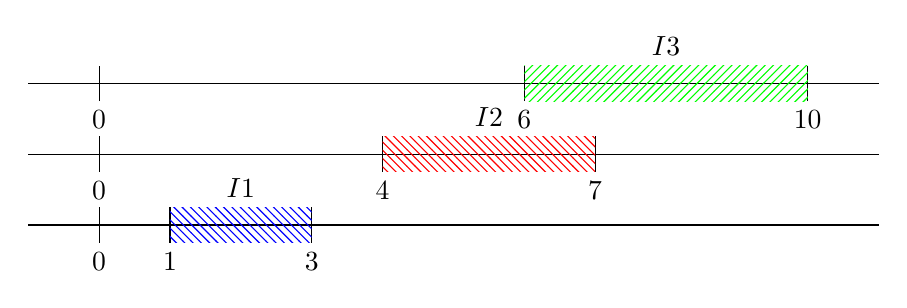
\begin{tikzpicture}[scale=0.9]
\draw (-1,0) -- (11,0) ;
\foreach \x in {0,1,3}
    {\draw (\x,-0.25) -- (\x, 0.25);
    \draw (\x,-0.25) node[below]{$\x$};}
\draw (2,0.25) node[above]{$I1$};
\fill [pattern=north west lines, pattern color=blue] (1,-0.25) rectangle (3,0.25);
\draw (-1,1) -- (11,1) ;
\foreach \x in {0,4,7}
    {\draw (\x,0.75) -- (\x, 1.25);
    \draw (\x,0.75) node[below]{$\x$};}
\draw (5.5,1.25) node[above]{$I2$};
\fill [pattern=north west lines, pattern color=red] (4,0.75) rectangle (7,1.25);
\draw (-1,2) -- (11,2) ;
\foreach \x in {0,6,10}
    {\draw (\x,1.75) -- (\x, 2.25);
    \draw (\x,1.75) node[below]{$\x$};}
\draw (8,2.25) node[above]{$I3$};
\fill [pattern=north east lines, pattern color=green] (6,1.75) rectangle (10,2.25);
\end{tikzpicture}
\end{block}
}

\only<3>{
\begin{block}{Example}
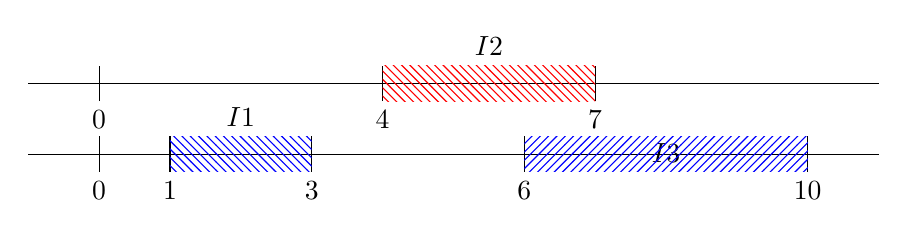
\begin{tikzpicture}[scale=0.9]
\draw (-1,0) -- (11,0) ;
\foreach \x in {0,1,3,6,10}
    {\draw (\x,-0.25) -- (\x, 0.25);
    \draw (\x,-0.25) node[below]{$\x$};}
\draw (2,0.25) node[above]{$I1$};
\fill [pattern=north west lines, pattern color=blue] (1,-0.25) rectangle (3,0.25);
\draw (8,-0.25) node[above]{$I3$};
\fill [pattern=north east lines, pattern color=blue] (6,-0.25) rectangle (10,0.25);
\draw (-1,1) -- (11,1) ;
\foreach \x in {0,4,7}
    {\draw (\x,0.75) -- (\x, 1.25);
    \draw (\x,0.75) node[below]{$\x$};}
\draw (5.5,1.25) node[above]{$I2$};
\fill [pattern=north west lines, pattern color=red] (4,0.75) rectangle (7,1.25);
\end{tikzpicture}
\end{block}
}
\end{overlayarea}

\end{frame}

\begin{frame}{Problem modelisation}

\begin{block}{Graph modelisation ...}
Undirected graph:
\begin{itemize}
\item[$\bullet$] each vertex is an interval;
\item[$\bullet$] each edge is the intersection between two intervals (the two vertices of this edge).
\end{itemize}
\end{block}
\pause
\begin{block}{... or intervals modelisation !}<2->
\begin{itemize}
\item[$\bullet$] An interval is defined by two endpoints: left and right.
\item[$\bullet$] Intervals are in a set, sorted by endpoints.
\end{itemize}
\end{block}

\end{frame}


\begin{frame}{More about graphs}

\begin{block}{Chordal graphs}
\alert{Def:} A chordal graph is a graph in which every cycle of four or more vertices have an extra edge connecting two node of the cycle.
\end{block}


\begin{block}{Interval graphs are chordal graphs}

\only<2>{
\begin{tabular}{lcr}
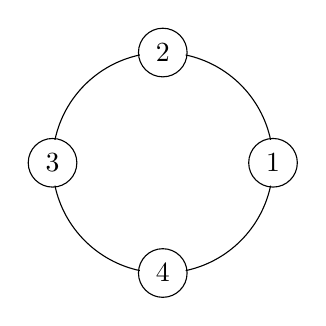
\begin{tikzpicture}
\def \margin {12}
\def \radius {1.4cm}
\def \n {4}
\foreach \s in {1,...,\n}
  {\node[draw, circle] at ({360/\n * (\s - 1)}:\radius) {$\s$};
   \draw ({360/\n * (\s - 1)+\margin}:\radius) 
    arc ({360/\n * (\s - 1)+\margin}:{360/\n * (\s)-\margin}:\radius);}
\end{tikzpicture}
&
\vspace{-2cm}
\begin{tikzpicture}
\draw[<->, red, very thick] (-0.5,1) -- (0.5,1);
\draw[white, ultra thin] (0,-0.5) -- (0,1);
\end{tikzpicture}
&
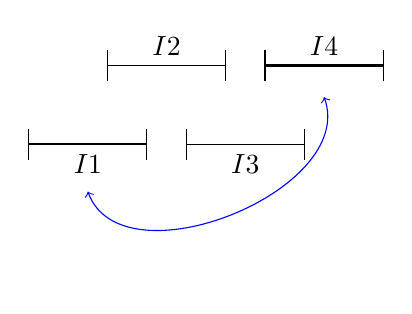
\begin{tikzpicture}
\foreach \x in {0,1.5,2,3.5}
    {\draw (\x,-0.2) -- (\x, 0.2);}
\draw (0.75,0) node[below]{$I1$};
\draw[thick] (0,0) -- (1.5,0);
\draw (2.75,0) node[below]{$I3$};
\draw (2,0) -- (3.5,0);

\foreach \x in {1,2.5,3,4.5}
    {\draw (\x,0.8) -- (\x, 1.2);}
\draw (1.75,1) node[above]{$I2$};
\draw (1,1) -- (2.5,1);
\draw (3.75,1) node[above]{$I4$};
\draw[thick] (3,1) -- (4.5,1);

\draw[<->,blue] (0.75,-0.6) to[out=290, in=290] (3.75,0.6);
\end{tikzpicture}
\end{tabular}
}

\only<3>{
\begin{tabular}{lcr}
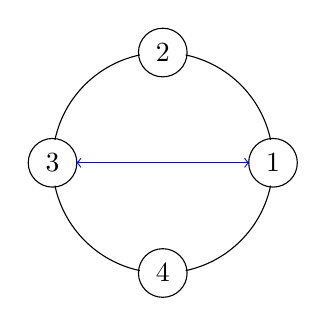
\begin{tikzpicture}
\def \margin {12}
\def \radius {1.4cm}
\def \n {4}
\foreach \s in {1,...,\n}
  {\node[draw, circle] at ({360/\n * (\s - 1)}:\radius) {$\s$};
   \draw ({360/\n * (\s - 1)+\margin}:\radius) 
    arc ({360/\n * (\s - 1)+\margin}:{360/\n * (\s)-\margin}:\radius);}
\draw[<->,blue] (-1.1,0) -- (1.1,0);
\end{tikzpicture}
&
\vspace{-2cm}
\begin{tikzpicture}
\draw[<->, green, very thick] (-0.5,1) -- (0.5,1);
\draw[white, ultra thin] (0,-0.5) -- (0,1);
\end{tikzpicture}
&
\begin{tikzpicture}
\foreach \x in {0,4}
    {\draw (\x,-0.2) -- (\x, 0.2);}
\draw (2,0) node[below]{$I1$};
\draw (0,0) -- (4,0);

\foreach \x in {2,3.5}
    {\draw (\x,-1.2) -- (\x, -0.8);}
\draw (2.75,-1) node[below]{$I3$};
\draw (2,-1) -- (3.5,-1);

\foreach \x in {1,2.5,3,4.5}
    {\draw (\x,0.8) -- (\x, 1.2);}
\draw (1.75,1) node[above]{$I2$};
\draw (1,1) -- (2.5,1);
\draw (3.75,1) node[above]{$I4$};
\draw (3,1) -- (4.5,1);

\end{tikzpicture}
\end{tabular}
}
\end{block}

\end{frame}



\section{Related Work}

\begin{frame}{Context}


\begin{block}{Related NP-complete problems}
Given an arbitrary graph $\mathnormal{G}$ and $\mathnormal{k}$ colors:
\begin{itemize}
\item[$\bullet$] is $\mathnormal{G}$ $\mathnormal{k}$-colorable ?
\item[$\bullet$] find a maximal $\mathnormal{k}$-colorable subgraph of $\mathnormal{G}$
\end{itemize}
\end{block}
\pause
\begin{block}{Related $\mathnormal{O(n + e)}$ problems, assuming that $\mathnormal{G}$ is \emph{chordal}}<2->
$\mathnormal{n}$ is the number of vertices, $\mathnormal{e}$ the number of edges.
\begin{itemize}
\item[$\bullet$] is $\mathnormal{G}$ $\mathnormal{k}$-colorable ?
\item[$\bullet$] find a maximal $\mathnormal{k}$-colorable subgraph of $G$
\end{itemize}
\end{block}
\pause
\begin{block}{Article's problem}<3->
\begin{itemize}
\item[$\bullet$] $\mathnormal{O(n + e)}$ with previous algorithm;
\item[$\bullet$] $\mathnormal{O(n~log~k)}$ if intervals are presorted by endpoints.
\end{itemize} 
\end{block}
\end{frame}



\section{Algorithm}

\begin{frame}{Working}
\begin{itemize}
\item[$\bullet$]Endpoints sorted
\item[$\bullet$]Intervals ordered by increasing right endpoint $\mathrm{I_{1}, I_{2},\dots,  I_{n}}$
\item[$\bullet$]Intervals processed in order using Greedy approach
\end{itemize}
\end{frame}

\begin{frame}{Processing an interval}

\begin{overlayarea}{\textwidth}{\textheight}
\vspace{0.5cm}
Two possibilities :
\begin{itemize}
\item[$\bullet$]If no available color, discard
\item[$\bullet$]Otherwise, assign best fitting color
\end{itemize}

Intuitively, best fit = closest available color on left-side

\vspace{2cm}

\only<2>{
    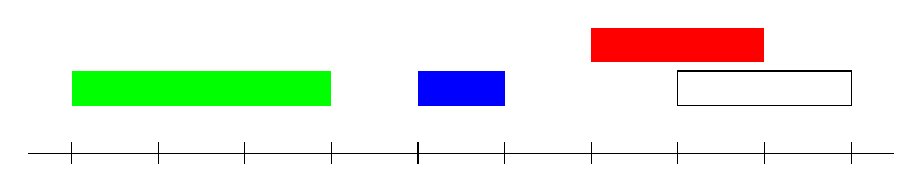
\begin{tikzpicture}[scale=0.55]
    \draw (-1,-1.5) -- (19,-1.5);
          \foreach \x in {0,2,...,18}
        {\draw (\x,-1.75) -- (\x, -1.25);}
    \fill[color=green] (0,-0.4) rectangle (6,0.4);
    \fill[color=blue] (8,-0.4) rectangle (10,0.4);
    \draw (14,-0.4) rectangle (18,0.4);
    \fill[color=red] (12,0.6) rectangle (16,1.40);
    \end{tikzpicture}
}

\only<3>{
    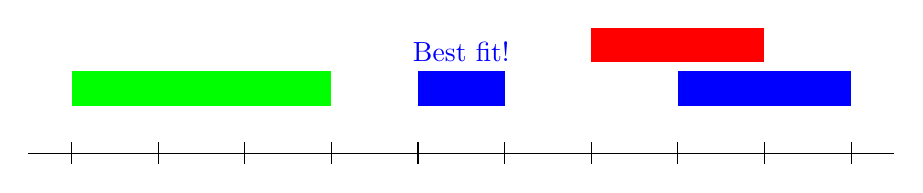
\begin{tikzpicture}[scale=0.55]
    \draw (-1,-1.5) -- (19,-1.5);
          \foreach \x in {0,2,...,18}
        {\draw (\x,-1.75) -- (\x, -1.25);}
    \fill[color=green] (0,-0.4) rectangle (6,0.4);
    \fill[color=blue] (8,-0.4) rectangle (10,0.4);
    \draw (9,0.4) node[above] {\textcolor{blue}{Best fit!}};
    \fill[color=blue] (14,-0.4) rectangle (18,0.4);
    \fill[color=red] (12,0.6) rectangle (16,1.40);
    \end{tikzpicture}
}

\end{overlayarea}
\end{frame}

\begin{frame}{Best fit}
\begin{definition}

%\vspace{0.3cm}
\textcolor{blue}{Leader} (color $\mathrm{k}$) : Interval of largest right endpoint with color $\mathrm{k}$\\

%\vspace{0.5cm}
\textcolor{blue}{Adjacent} (interval $\mathrm{I_{i}}$) : Interval of greatest right endpoint no greater than $\mathrm{I_{i}}$'s left endpoint\\

%\vspace{0.5cm}
\textcolor{blue}{Best fit leader} (interval $\mathrm{I_{i}}$) : Leader of greatest right endpoint no greater than $\mathrm{I_{i}}$'s left endpoint
\end{definition}

Best fit color for $\mathrm{I_{i}}$ = color Best\_fit\_leader($I_{i}$)

%TODO : rajouter que le best fit leader se trouve en O(1) en amortized complexity analysis
\end{frame}

\begin{frame}{Interval sets}
  \begin{itemize}
    %\item[$\bullet$]Grouping intervals by sets representing equivalence classes with respect to "best fits"
    \item[$\bullet$]Interval of least index gives its name to the set. In fact, it's a leader
    \item[$\bullet$]At any time, only 1 leader per set
    \item[$\bullet$]\texttt{find($\mathrm{I}$)} : returns the leader of the set of $\mathrm{I}$
    \item[$\bullet$]Best fit leader : \texttt{find(adjacent($\mathrm{I}$))}
\item[$\bullet$]During the algorithm : unions of sets
    %\item[$\bullet$]Processing : \texttt{if} $\mathrm{I_{j}}$ is discarded \textbf{or} not a leader, \texttt{then} set($\mathrm{I_{j}}$) $\cup$ set($\mathrm{I_{j-1}}$)
    \item[$\bullet$]Initially : singleton sets
  \end{itemize}
\end{frame}
\begin{frame}{Example}
\begin{overlayarea}{\textwidth}{\textheight}

  \only<1>{
    \vspace{1cm}
    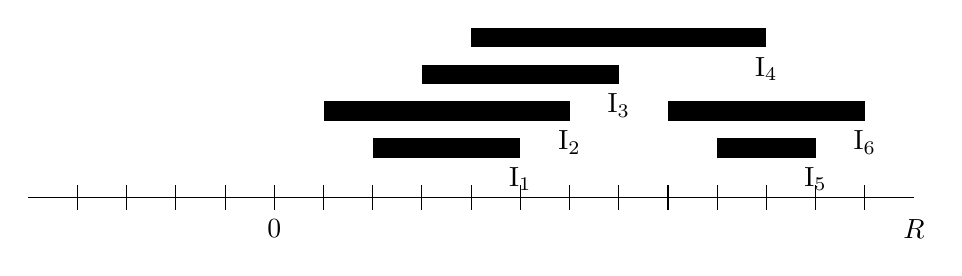
\begin{tikzpicture}[scale=0.625]
      \draw (-5,0) -- (13,0);
      \draw (13,-0.25) node[below]{$\mathbb{R}$};
      \draw (0,-0.25) node[below]{0};
      \foreach \x in {-4,-3,...,12}
        {\draw (\x,-0.25) -- (\x, 0.25);}

      \fill (2,0.80) rectangle (5,1.20);
      \draw (5, 0.80) node[below]{$\mathrm{I_{1}}$};
      \fill (1,1.55) rectangle (6,1.95);
      \draw (6, 1.55) node[below]{$\mathrm{I_{2}}$};
      \fill (3,2.30) rectangle (7,2.70);
      \draw (7, 2.30) node[below]{$\mathrm{I_{3}}$};
      \fill (4,3.05) rectangle (10,3.45);
      \draw (10, 3.05) node[below]{$\mathrm{I_{4}}$};
      \fill (9,0.80) rectangle (11,1.20);
      \draw (11, 0.80) node[below]{$\mathrm{I_{5}}$};
      \fill (8,1.55) rectangle (12,1.95);
      \draw (12, 1.55) node[below]{$\mathrm{I_{6}}$};
    \end{tikzpicture}
  }

  \only<2>{
      \vspace{1cm}
    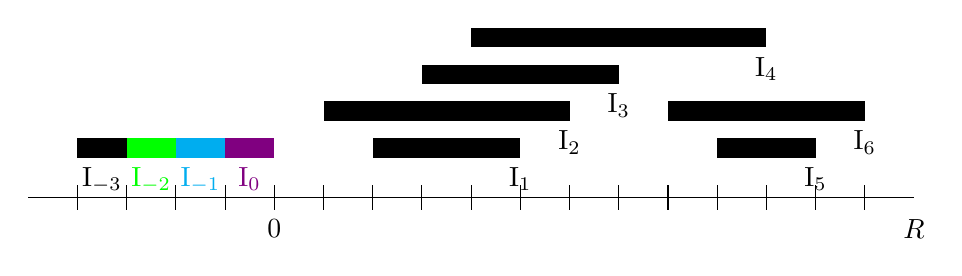
\begin{tikzpicture}[scale=0.625]
      \draw (-5,0) -- (13,0);
      \draw (13,-0.25) node[below]{$\mathbb{R}$};
      \draw (0,-0.25) node[below]{0};
      \foreach \x in {-4,-3,...,12}
        {\draw (\x,-0.25) -- (\x, 0.25);}

      \fill (-4,0.80) rectangle (-3,1.20);
      \draw (-3.5, 0.80) node[below]{$\mathrm{I_{-3}}$};
      \fill[color = green] (-3,0.80) rectangle (-2,1.20);
      \draw (-2.5, 0.80) node[below]{\textcolor{green}{$\mathrm{I_{-2}}$}};
      \fill[color = cyan] (-2,0.80) rectangle (-1,1.20);
      \draw (-1.5, 0.80) node[below]{\textcolor{cyan}{$\mathrm{I_{-1}}$}};
      \fill[color = violet] (-1,0.80) rectangle (0,1.20);
      \draw (-0.5, 0.80) node[below]{\textcolor{violet}{$\mathrm{I_{0}}$}};
      \fill (2,0.80) rectangle (5,1.20);
      \draw (5, 0.80) node[below]{$\mathrm{I_{1}}$};
      \fill (1,1.55) rectangle (6,1.95);
      \draw (6, 1.55) node[below]{$\mathrm{I_{2}}$};
      \fill (3,2.30) rectangle (7,2.70);
      \draw (7, 2.30) node[below]{$\mathrm{I_{3}}$};
      \fill (4,3.05) rectangle (10,3.45);
      \draw (10, 3.05) node[below]{$\mathrm{I_{4}}$};
      \fill (9,0.80) rectangle (11,1.20);
      \draw (11, 0.80) node[below]{$\mathrm{I_{5}}$};
      \fill (8,1.55) rectangle (12,1.95);
      \draw (12, 1.55) node[below]{$\mathrm{I_{6}}$};
    \end{tikzpicture}
    \begin{block}{Sets}
    \{$\mathrm{I_{-3}}$\} \{\textcolor{green}{$\mathrm{I_{-2}}$}\} \{\textcolor{cyan}{$\mathrm{I_{-1}}$}\} \{\textcolor{violet}{$\mathrm{I_{0}}$}\} \{$\mathrm{I_{1}}$\} \{$\mathrm{I_{2}}$\} \{$\mathrm{I_{3}}$\} \{$\mathrm{I_{4}}$\} \{$\mathrm{I_{5}}$\} \{$\mathrm{I_{6}}$\}
    \end{block}
  }

  \only<3>{
      \vspace{1cm}
    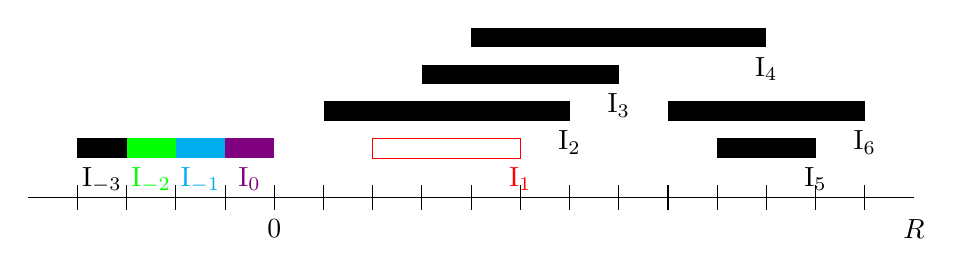
\begin{tikzpicture}[scale=0.625]
      \draw (-5,0) -- (13,0);
      \draw (13,-0.25) node[below]{$\mathbb{R}$};
      \draw (0,-0.25) node[below]{0};
      \foreach \x in {-4,-3,...,12}
        {\draw (\x,-0.25) -- (\x, 0.25);}

      \fill (-4,0.80) rectangle (-3,1.20);
      \draw (-3.5, 0.80) node[below]{$\mathrm{I_{-3}}$};
      \fill[color = green] (-3,0.80) rectangle (-2,1.20);
      \draw (-2.5, 0.80) node[below]{\textcolor{green}{$\mathrm{I_{-2}}$}};
      \fill[color = cyan] (-2,0.80) rectangle (-1,1.20);
      \draw (-1.5, 0.80) node[below]{\textcolor{cyan}{$\mathrm{I_{-1}}$}};
      \fill[color = violet] (-1,0.80) rectangle (0,1.20);
      \draw (-0.5, 0.80) node[below]{\textcolor{violet}{$\mathrm{I_{0}}$}};
      \draw [color = red] (2,0.80) rectangle (5,1.20);
      \draw (5, 0.80) node[below]{\textcolor{red}{$\mathrm{I_{1}}$}};
      \fill (1,1.55) rectangle (6,1.95);
      \draw (6, 1.55) node[below]{$\mathrm{I_{2}}$};
      \fill (3,2.30) rectangle (7,2.70);
      \draw (7, 2.30) node[below]{$\mathrm{I_{3}}$};
      \fill (4,3.05) rectangle (10,3.45);
      \draw (10, 3.05) node[below]{$\mathrm{I_{4}}$};
      \fill (9,0.80) rectangle (11,1.20);
      \draw (11, 0.80) node[below]{$\mathrm{I_{5}}$};
      \fill (8,1.55) rectangle (12,1.95);
      \draw (12, 1.55) node[below]{$\mathrm{I_{6}}$};
    \end{tikzpicture}
    \begin{block}{Sets}
    \{$\mathrm{I_{-3}}$\} \{\textcolor{green}{$\mathrm{I_{-2}}$}\} \{\textcolor{cyan}{$\mathrm{I_{-1}}$}\} \{\textcolor{violet}{$\mathrm{I_{0}}$}\} \{$\mathrm{I_{1}}$\} \{$\mathrm{I_{2}}$\} \{$\mathrm{I_{3}}$\} \{$\mathrm{I_{4}}$\} \{$\mathrm{I_{5}}$\} \{$\mathrm{I_{6}}$\}
    \end{block}
    \begin{block}{Operations}
      \begin{columns}[T]
      \begin{column}{.48\textwidth}
        \begin{itemize}
          \item[$\bullet$]i = 1
          \item[$\bullet$]adjacent($\mathrm{I_{i}}$) = $\mathrm{I_{0}}$
          \item[$\bullet$]Best fit leader = find(adjacent($\mathrm{I_{i}}$)) = $\mathrm{I_{0}}$
        \end{itemize}
      \end{column}
      \begin{column}{.48\textwidth}
        \begin{itemize}
          \item[\textcolor{red}{$\bullet$}]\textcolor{red}{color($\mathrm{I_{i}}$)$\leftarrow$color($\mathrm{I_{j}}$)}
          \item[$\bullet$]find($\mathrm{I_{j-1}}$) = $\mathrm{I_{-1}}$
          \item[\textcolor{red}{$\bullet$}]\textcolor{red}{union($\mathrm{I_{j}}$,find($\mathrm{I_{j-1}}$))}
        \end{itemize}
      \end{column}
      \end{columns}  
    \end{block}
  }
    \only<4>{
    \vspace{1cm}
    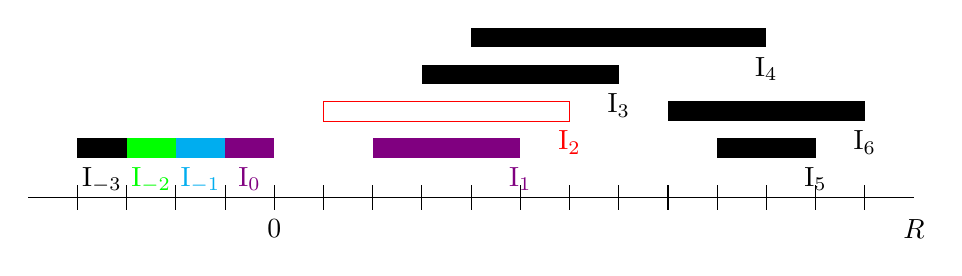
\begin{tikzpicture}[scale=0.625]
      \draw (-5,0) -- (13,0);
      \draw (13,-0.25) node[below]{$\mathbb{R}$};
      \draw (0,-0.25) node[below]{0};
      \foreach \x in {-4,-3,...,12}
        {\draw (\x,-0.25) -- (\x, 0.25);}

      \fill (-4,0.80) rectangle (-3,1.20);
      \draw (-3.5, 0.80) node[below]{$\mathrm{I_{-3}}$};
      \fill[color=green] (-3,0.80) rectangle (-2,1.20);
      \draw (-2.5, 0.80) node[below]{\textcolor{green}{$\mathrm{I_{-2}}$}};
      \fill[color=cyan] (-2,0.80) rectangle (-1,1.20);
      \draw (-1.5, 0.80) node[below]{\textcolor{cyan}{$\mathrm{I_{-1}}$}};
      \fill[color=violet] (-1,0.80) rectangle (0,1.20);
      \draw (-0.5, 0.80) node[below]{\textcolor{violet}{$\mathrm{I_{0}}$}};
      \fill[color=violet] (2,0.80) rectangle (5,1.20);
      \draw (5, 0.80) node[below]{\textcolor{violet}{$\mathrm{I_{1}}$}};
      \draw[color=red] (1,1.55) rectangle (6,1.95);
      \draw (6, 1.55) node[below]{\textcolor{red}{$\mathrm{I_{2}}$}};
      \fill (3,2.30) rectangle (7,2.70);
      \draw (7, 2.30) node[below]{$\mathrm{I_{3}}$};
      \fill (4,3.05) rectangle (10,3.45);
      \draw (10, 3.05) node[below]{$\mathrm{I_{4}}$};
      \fill (9,0.80) rectangle (11,1.20);
      \draw (11, 0.80) node[below]{$\mathrm{I_{5}}$};
      \fill (8,1.55) rectangle (12,1.95);
      \draw (12, 1.55) node[below]{$\mathrm{I_{6}}$};
    \end{tikzpicture}
    \begin{block}{Sets}
    \{$\mathrm{I_{-3}}$\} \{\textcolor{green}{$\mathrm{I_{-2}}$}\} \{\textcolor{cyan}{$\mathrm{I_{-1}}$},\textcolor{violet}{$\mathrm{I_{0}}$}\} \{\textcolor{violet}{$\mathrm{I_{1}}$}\} \{$\mathrm{I_{2}}$\} \{$\mathrm{I_{3}}$\} \{$\mathrm{I_{4}}$\} \{$\mathrm{I_{5}}$\} \{$\mathrm{I_{6}}$\}
    \end{block}
    \begin{block}{Operations}
      \begin{columns}[T]
      \begin{column}{.48\textwidth}
        \begin{itemize}
          \item[$\bullet$]i = 2
          \item[$\bullet$]adjacent($\mathrm{I_{2}}$) = $\mathrm{I_{0}}$
          \item[$\bullet$]find($\mathrm{I_{0}}$) = $\mathrm{I_{-1}}$
        \end{itemize}
      \end{column}
      \begin{column}{.48\textwidth}
        \begin{itemize}
          \item[\textcolor{red}{$\bullet$}]\textcolor{red}{color($\mathrm{I_{2}}$)$\leftarrow$color($\mathrm{I_{-1}}$)}
          \item[$\bullet$]find($\mathrm{I_{-2}}$) = $\mathrm{I_{-2}}$
          \item[\textcolor{red}{$\bullet$}]\textcolor{red}{union($\mathrm{I_{-1}},\mathrm{I_{-2}}$)}
        \end{itemize}
      \end{column}
      \end{columns}  
    \end{block}
  }
  
  \only<5>{
    \vspace{1cm}
    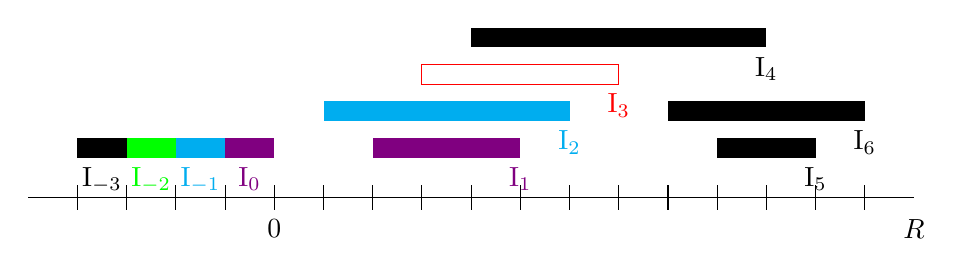
\begin{tikzpicture}[scale=0.625]
      \draw (-5,0) -- (13,0);
      \draw (13,-0.25) node[below]{$\mathbb{R}$};
      \draw (0,-0.25) node[below]{0};
      \foreach \x in {-4,-3,...,12}
        {\draw (\x,-0.25) -- (\x, 0.25);}

      \fill (-4,0.80) rectangle (-3,1.20);
      \draw (-3.5, 0.80) node[below]{$\mathrm{I_{-3}}$};
      \fill[color=green] (-3,0.80) rectangle (-2,1.20);
      \draw (-2.5, 0.80) node[below]{\textcolor{green}{$\mathrm{I_{-2}}$}};
      \fill[color=cyan] (-2,0.80) rectangle (-1,1.20);
      \draw (-1.5, 0.80) node[below]{\textcolor{cyan}{$\mathrm{I_{-1}}$}};
      \fill[color=violet] (-1,0.80) rectangle (0,1.20);
      \draw (-0.5, 0.80) node[below]{\textcolor{violet}{$\mathrm{I_{0}}$}};
      \fill[color=violet] (2,0.80) rectangle (5,1.20);
      \draw (5, 0.80) node[below]{\textcolor{violet}{$\mathrm{I_{1}}$}};
      \fill[color=cyan] (1,1.55) rectangle (6,1.95);
      \draw (6, 1.55) node[below]{\textcolor{cyan}{$\mathrm{I_{2}}$}};
      \draw[color=red] (3,2.30) rectangle (7,2.70);
      \draw (7, 2.30) node[below]{\textcolor{red}{$\mathrm{I_{3}}$}};
      \fill (4,3.05) rectangle (10,3.45);
      \draw (10, 3.05) node[below]{$\mathrm{I_{4}}$};
      \fill (9,0.80) rectangle (11,1.20);
      \draw (11, 0.80) node[below]{$\mathrm{I_{5}}$};
      \fill (8,1.55) rectangle (12,1.95);
      \draw (12, 1.55) node[below]{$\mathrm{I_{6}}$};
    \end{tikzpicture}
    \begin{block}{Sets}
    \{$\mathrm{I_{-3}}$\} \{\textcolor{green}{$\mathrm{I_{-2}}$},\textcolor{cyan}{$\mathrm{I_{-1}}$},\textcolor{violet}{$\mathrm{I_{0}}$}\} \{\textcolor{violet}{$\mathrm{I_{1}}$}\} \{\textcolor{cyan}{$\mathrm{I_{2}}$}\} \{$\mathrm{I_{3}}$\} \{$\mathrm{I_{4}}$\} \{$\mathrm{I_{5}}$\} \{$\mathrm{I_{6}}$\}
    \end{block}
    \begin{block}{Operations}
      \begin{columns}[T]
      \begin{column}{.48\textwidth}
        \begin{itemize}
          \item[$\bullet$]i = 3
          \item[$\bullet$]adjacent($\mathrm{I_{3}}$) = $\mathrm{I_{0}}$
          \item[$\bullet$]find($\mathrm{I_{0}}$) = $\mathrm{I_{-2}}$
        \end{itemize}
      \end{column}
      \begin{column}{.48\textwidth}
        \begin{itemize}
          \item[\textcolor{red}{$\bullet$}]\textcolor{red}{color($\mathrm{I_{3}}$)$\leftarrow$color($\mathrm{I_{-2}}$)}
          \item[$\bullet$]find($\mathrm{I_{-3}}$) = $\mathrm{I_{-3}}$
          \item[\textcolor{red}{$\bullet$}]\textcolor{red}{union($\mathrm{I_{-2}},\mathrm{I_{-3}}$)}
        \end{itemize}
      \end{column}
      \end{columns}  
    \end{block}
  }
  
  
    \only<6>{
    \vspace{1cm}
    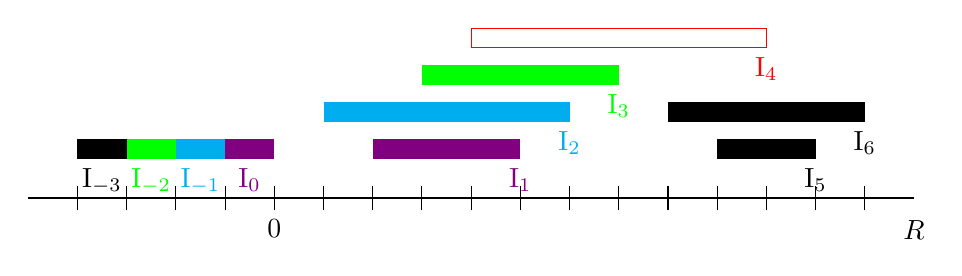
\begin{tikzpicture}[scale=0.625]
      \draw (-5,0) -- (13,0);
      \draw (13,-0.25) node[below]{$\mathbb{R}$};
      \draw (0,-0.25) node[below]{0};
      \foreach \x in {-4,-3,...,12}
        {\draw (\x,-0.25) -- (\x, 0.25);}

      \fill (-4,0.80) rectangle (-3,1.20);
      \draw (-3.5, 0.80) node[below]{$\mathrm{I_{-3}}$};
      \fill[color=green] (-3,0.80) rectangle (-2,1.20);
      \draw (-2.5, 0.80) node[below]{\textcolor{green}{$\mathrm{I_{-2}}$}};
      \fill[color=cyan] (-2,0.80) rectangle (-1,1.20);
      \draw (-1.5, 0.80) node[below]{\textcolor{cyan}{$\mathrm{I_{-1}}$}};
      \fill[color=violet] (-1,0.80) rectangle (0,1.20);
      \draw (-0.5, 0.80) node[below]{\textcolor{violet}{$\mathrm{I_{0}}$}};
      \fill[color=violet] (2,0.80) rectangle (5,1.20);
      \draw (5, 0.80) node[below]{\textcolor{violet}{$\mathrm{I_{1}}$}};
      \fill[color=cyan] (1,1.55) rectangle (6,1.95);
      \draw (6, 1.55) node[below]{\textcolor{cyan}{$\mathrm{I_{2}}$}};
      \fill[color=green] (3,2.30) rectangle (7,2.70);
      \draw (7, 2.30) node[below]{\textcolor{green}{$\mathrm{I_{3}}$}};
      \draw[color=red] (4,3.05) rectangle (10,3.45);
      \draw (10, 3.05) node[below]{\textcolor{red}{$\mathrm{I_{4}}$}};
      \fill (9,0.80) rectangle (11,1.20);
      \draw (11, 0.80) node[below]{$\mathrm{I_{5}}$};
      \fill (8,1.55) rectangle (12,1.95);
      \draw (12, 1.55) node[below]{$\mathrm{I_{6}}$};
    \end{tikzpicture}
    \begin{block}{Sets}
    \{$\mathrm{I_{-3}}$,\textcolor{green}{$\mathrm{I_{-2}}$},\textcolor{cyan}{$\mathrm{I_{-1}}$},\textcolor{violet}{$\mathrm{I_{0}}$}\} \{\textcolor{violet}{$\mathrm{I_{1}}$}\} \{\textcolor{cyan}{$\mathrm{I_{2}}$}\} \{\textcolor{green}{$\mathrm{I_{3}}$}\} \{$\mathrm{I_{4}}$\} \{$\mathrm{I_{5}}$\} \{$\mathrm{I_{6}}$\}
    \end{block}
    \begin{block}{Operations}
      \begin{columns}[T]
      \begin{column}{.48\textwidth}
        \begin{itemize}
          \item[$\bullet$]i = 4
          \item[$\bullet$]adjacent($\mathrm{I_{4}}$) = $\mathrm{I_{0}}$
          \item[$\bullet$]find($\mathrm{I_{0}}$) = $\mathrm{I_{-3}}$
        \end{itemize}
      \end{column}
      \begin{column}{.48\textwidth}
        \begin{itemize}
          \item[\textcolor{red}{$\bullet$}]\textcolor{red}{color($\mathrm{I_{4}}$)$\leftarrow$0}
          \item[$\bullet$]find($\mathrm{I_{i-1}}$) = $\mathrm{I_{3}}$
          \item[\textcolor{red}{$\bullet$}]\textcolor{red}{union($\mathrm{I_{i}}$,find($\mathrm{I_{i-1}}$))}
        \end{itemize}
      \end{column}
      \end{columns}  
    \end{block}
  }
  
      \only<7>{
    \vspace{1cm}
    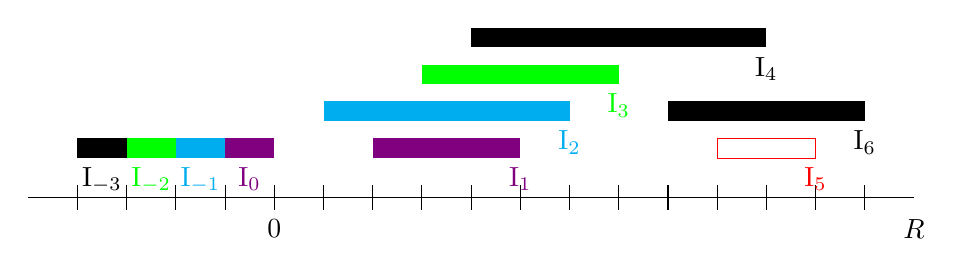
\begin{tikzpicture}[scale=0.625]
      \draw (-5,0) -- (13,0);
      \draw (13,-0.25) node[below]{$\mathbb{R}$};
      \draw (0,-0.25) node[below]{0};
      \foreach \x in {-4,-3,...,12}
        {\draw (\x,-0.25) -- (\x, 0.25);}

      \fill (-4,0.80) rectangle (-3,1.20);
      \draw (-3.5, 0.80) node[below]{$\mathrm{I_{-3}}$};
      \fill[color=green] (-3,0.80) rectangle (-2,1.20);
      \draw (-2.5, 0.80) node[below]{\textcolor{green}{$\mathrm{I_{-2}}$}};
      \fill[color=cyan] (-2,0.80) rectangle (-1,1.20);
      \draw (-1.5, 0.80) node[below]{\textcolor{cyan}{$\mathrm{I_{-1}}$}};
      \fill[color=violet] (-1,0.80) rectangle (0,1.20);
      \draw (-0.5, 0.80) node[below]{\textcolor{violet}{$\mathrm{I_{0}}$}};
      \fill[color=violet] (2,0.80) rectangle (5,1.20);
      \draw (5, 0.80) node[below]{\textcolor{violet}{$\mathrm{I_{1}}$}};
      \fill[color=cyan] (1,1.55) rectangle (6,1.95);
      \draw (6, 1.55) node[below]{\textcolor{cyan}{$\mathrm{I_{2}}$}};
      \fill[color=green] (3,2.30) rectangle (7,2.70);
      \draw (7, 2.30) node[below]{\textcolor{green}{$\mathrm{I_{3}}$}};
      \fill (4,3.05) rectangle (10,3.45);
      \draw (10, 3.05) node[below]{$\mathrm{I_{4}}$};
      \draw[color=red] (9,0.80) rectangle (11,1.20);
      \draw (11, 0.80) node[below]{\textcolor{red}{$\mathrm{I_{5}}$}};
      \fill (8,1.55) rectangle (12,1.95);
      \draw (12, 1.55) node[below]{$\mathrm{I_{6}}$};
    \end{tikzpicture}
    \begin{block}{Sets}
    \{$\mathrm{I_{-3}}$,\textcolor{green}{$\mathrm{I_{-2}}$},\textcolor{cyan}{$\mathrm{I_{-1}}$},\textcolor{violet}{$\mathrm{I_{0}}$}\} \{\textcolor{violet}{$\mathrm{I_{1}}$}\} \{\textcolor{cyan}{$\mathrm{I_{2}}$}\} \{\textcolor{green}{$\mathrm{I_{3}}$},$\mathrm{I_{4}}$\} \{$\mathrm{I_{5}}$\} \{$\mathrm{I_{6}}$\}
    \end{block}
    \begin{block}{Operations}
      \begin{columns}[T]
      \begin{column}{.48\textwidth}
        \begin{itemize}
          \item[$\bullet$]i = 5
          \item[$\bullet$]adjacent($\mathrm{I_{5}}$) = $\mathrm{I_{3}}$
          \item[$\bullet$]find($\mathrm{I_{3}}$) = $\mathrm{I_{3}}$
        \end{itemize}
      \end{column}
      \begin{column}{.48\textwidth}
        \begin{itemize}
          \item[\textcolor{red}{$\bullet$}]\textcolor{red}{color($\mathrm{I_{5}}$)$\leftarrow$color($\mathrm{I_{3}}$)}
          \item[$\bullet$]find($\mathrm{I_{2}}$) = $\mathrm{I_{2}}$
          \item[\textcolor{red}{$\bullet$}]\textcolor{red}{union($\mathrm{I_{3}}$,find($\mathrm{I_{2}}$))}
        \end{itemize}
      \end{column}
      \end{columns}  
    \end{block}
  }
  
   
   \only<8>{
    \vspace{1cm}
    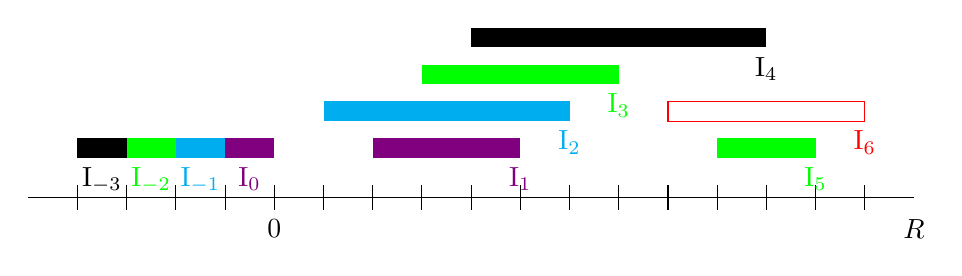
\begin{tikzpicture}[scale=0.625]
      \draw (-5,0) -- (13,0);
      \draw (13,-0.25) node[below]{$\mathbb{R}$};
      \draw (0,-0.25) node[below]{0};
      \foreach \x in {-4,-3,...,12}
        {\draw (\x,-0.25) -- (\x, 0.25);}

      \fill (-4,0.80) rectangle (-3,1.20);
      \draw (-3.5, 0.80) node[below]{$\mathrm{I_{-3}}$};
      \fill[color=green] (-3,0.80) rectangle (-2,1.20);
      \draw (-2.5, 0.80) node[below]{\textcolor{green}{$\mathrm{I_{-2}}$}};
      \fill[color=cyan] (-2,0.80) rectangle (-1,1.20);
      \draw (-1.5, 0.80) node[below]{\textcolor{cyan}{$\mathrm{I_{-1}}$}};
      \fill[color=violet] (-1,0.80) rectangle (0,1.20);
      \draw (-0.5, 0.80) node[below]{\textcolor{violet}{$\mathrm{I_{0}}$}};
      \fill[color=violet] (2,0.80) rectangle (5,1.20);
      \draw (5, 0.80) node[below]{\textcolor{violet}{$\mathrm{I_{1}}$}};
      \fill[color=cyan] (1,1.55) rectangle (6,1.95);
      \draw (6, 1.55) node[below]{\textcolor{cyan}{$\mathrm{I_{2}}$}};
      \fill[color=green] (3,2.30) rectangle (7,2.70);
      \draw (7, 2.30) node[below]{\textcolor{green}{$\mathrm{I_{3}}$}};
      \fill (4,3.05) rectangle (10,3.45);
      \draw (10, 3.05) node[below]{$\mathrm{I_{4}}$};
      \fill[color=green] (9,0.80) rectangle (11,1.20);
      \draw (11, 0.80) node[below]{\textcolor{green}{$\mathrm{I_{5}}$}};
      \draw[color=red] (8,1.55) rectangle (12,1.95);
      \draw (12, 1.55) node[below]{\textcolor{red}{$\mathrm{I_{6}}$}};
    \end{tikzpicture}
    \begin{block}{Sets}
    \{$\mathrm{I_{-3}}$,\textcolor{green}{$\mathrm{I_{-2}}$},\textcolor{cyan}{$\mathrm{I_{-1}}$},\textcolor{violet}{$\mathrm{I_{0}}$}\} \{\textcolor{violet}{$\mathrm{I_{1}}$}\} \{\textcolor{cyan}{$\mathrm{I_{2}}$},\textcolor{green}{$\mathrm{I_{3}}$},$\mathrm{I_{4}}$\} \{\textcolor{green}{$\mathrm{I_{5}}$}\} \{$\mathrm{I_{6}}$\}
    \end{block}
    \begin{block}{Operations}
      \begin{columns}[T]
      \begin{column}{.48\textwidth}
        \begin{itemize}
          \item[$\bullet$]i = 6
          \item[$\bullet$]adjacent($\mathrm{I_{6}}$) = $\mathrm{I_{3}}$
          \item[$\bullet$]find($\mathrm{I_{3}}$) = $\mathrm{I_{2}}$
        \end{itemize}
      \end{column}
      \begin{column}{.48\textwidth}
        \begin{itemize}
          \item[\textcolor{red}{$\bullet$}]\textcolor{red}{color($\mathrm{I_{6}}$)$\leftarrow$color($\mathrm{I_{2}}$)}
          \item[$\bullet$]find($\mathrm{I_{1}}$) = $\mathrm{I_{1}}$
          \item[\textcolor{red}{$\bullet$}]\textcolor{red}{union($\mathrm{I_{2}}$,find($\mathrm{I_{1}}$))}
        \end{itemize}
      \end{column}
      \end{columns}  
    \end{block}
  }
  
  
     \only<9>{
    \vspace{1cm}
    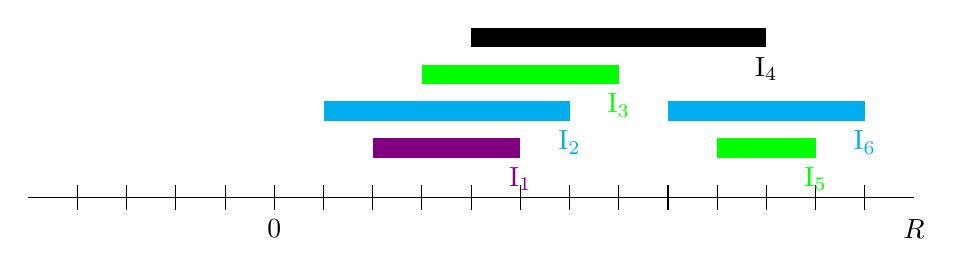
\begin{tikzpicture}[scale=0.625]
      \draw (-5,0) -- (13,0);
      \draw (13,-0.25) node[below]{$\mathbb{R}$};
      \draw (0,-0.25) node[below]{0};
      \foreach \x in {-4,-3,...,12}
        {\draw (\x,-0.25) -- (\x, 0.25);}

      \fill[color=violet] (2,0.80) rectangle (5,1.20);
      \draw (5, 0.80) node[below]{\textcolor{violet}{$\mathrm{I_{1}}$}};
      \fill[color=cyan] (1,1.55) rectangle (6,1.95);
      \draw (6, 1.55) node[below]{\textcolor{cyan}{$\mathrm{I_{2}}$}};
      \fill[color=green] (3,2.30) rectangle (7,2.70);
      \draw (7, 2.30) node[below]{\textcolor{green}{$\mathrm{I_{3}}$}};
      \fill (4,3.05) rectangle (10,3.45);
      \draw (10, 3.05) node[below]{$\mathrm{I_{4}}$};
      \fill[color=green] (9,0.80) rectangle (11,1.20);
      \draw (11, 0.80) node[below]{\textcolor{green}{$\mathrm{I_{5}}$}};
      \fill[color=cyan] (8,1.55) rectangle (12,1.95);
      \draw (12, 1.55) node[below]{\textcolor{cyan}{$\mathrm{I_{6}}$}};
    \end{tikzpicture}
    \begin{block}{Sets}
    \{$\mathrm{I_{-3}}$,\textcolor{green}{$\mathrm{I_{-2}}$},\textcolor{cyan}{$\mathrm{I_{-1}}$},\textcolor{violet}{$\mathrm{I_{0}}$}\} \{\textcolor{violet}{$\mathrm{I_{1}}$},\textcolor{cyan}{$\mathrm{I_{2}}$},\textcolor{green}{$\mathrm{I_{3}}$},$\mathrm{I_{4}}$\} \{\textcolor{green}{$\mathrm{I_{5}}$}\} \{\textcolor{cyan}{$\mathrm{I_{6}}$}\}
    \end{block}
  }
  
\end{overlayarea}
\end{frame}
\begin{frame}{Complexity : $O(n+k)$}
            \begin{algorithmic}
                \footnotesize
                \For{$i\gets 0$ to $k$}\Comment{\textcolor{red}{initialize dummy intervals : $O(k)$}}
                    \State\Call{right}{$I_{-i}$} $\gets -i$
                    \State\Call{left}{$I_{-i}$} $\gets -i-1$
                    \State\Call{color}{$I_{-i}$} $\gets k-i$
                    \State create a singleton set containing $I_{-i}$
                \EndFor
                \For{$i\gets 1$ to $n$}\Comment{\textcolor{red}{setup adjacent, and the sets : $O(n)$}}
                    \State\Call{adjacent}{$I_{i}$}$\gets$\Call{max}{j; \Call{right}{$I_{j}$}$\leq$\Call{left}{$I_{i}$}}
                    \State create a singleton set containing $I_{i}$
                \EndFor
                \For{$i\gets 1$ to $n$}\Comment{\textcolor{red}{main loop : $O(n)$}}
                    \State $I_{j}\gets$\Call{find}{\Call{adjacent}{$I_{i}$}}
                    \If{$j=-k$}
                        \State\Call{color}{$I_{i}$}$\gets 0$
                        \State\Call{union}{$I_{i}$,\Call{find}{$I_{i-1}$}}
                    \Else
                        \State\Call{color}{$I_{i}$}$\gets$\Call{color}{$I_{j}$}
                        \State\Call{union}{$I_{j}$,\Call{find}{$I_{j-1}$}}\Comment{\textcolor{red}{union done in constant time}}
                    \EndIf
                \EndFor
            \end{algorithmic}
\end{frame}
\begin{frame}{Weighted}
\begin{itemize}
\item[$\bullet$]Each interval has a positive weight
\item[$\bullet$]Goal : given $k$ colors, find a coloring maximizing the total weight
\item[$\bullet$]Idea : reducing the problem to a network flow problem (minimum cost flow)
\end{itemize}
\end{frame}

\begin{frame}{From intervals to network}
\begin{itemize}
\item[$\bullet$]Endpoints sorted $\mathrm{x_{1}<x_{2}<\dots<x_{r}}$
\item[$\bullet$]Intervals sorted by increasing right endpoints $\mathrm{I_{1}, I_{2},\dots,  I_{n}}$
\item[$\bullet$]Construction of the network
    \begin{itemize}
    \item Vertices : $\mathrm{s=v_{0},\ \ v_{1},\ \dots, v_{r},\ \ v_{r+1}=t}$
    \item Clique-edges between $\mathrm{(v_{i},v_{i+1})}$ with $\mathrm{cost = 0}$ and $\mathrm{capacity = k}$
    \item Interval-edges between the two endpoints of an interval with $\mathrm{cost = -1 \times weight}$ and $\mathrm{capacity = 1}$
    \end{itemize}
\item[$\bullet$]1 unit of flow = 1 color
\end{itemize}
\end{frame}

\begin{frame}{Example}
\begin{overlayarea}{\textwidth}{\textheight}

\only<1>{
\vspace{0.5cm}
Number of colors = 2
\vspace{0.2cm}

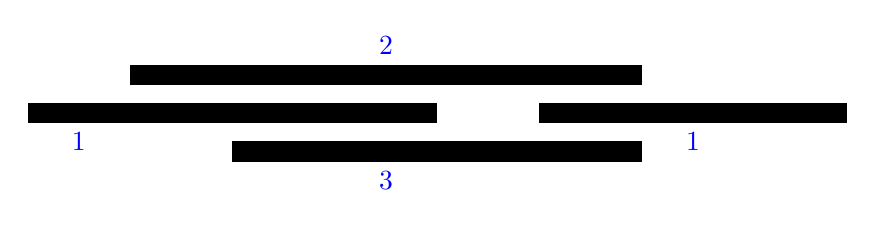
\begin{tikzpicture}[scale=0.65]

\fill (0,0.55) rectangle (8,0.95);
\draw (1, 0.55) node[below]{\textcolor{blue}{$1$}};

\fill (2,1.3) rectangle (12,1.7);
\draw (7, 1.7) node[above]{\textcolor{blue}{$2$}};

\fill (4,-0.2) rectangle (12,0.2);
\draw (7, -0.2) node[below]{\textcolor{blue}{$3$}};

\fill (10,0.55) rectangle (16,0.95);
\draw (13, 0.55) node[below]{\textcolor{blue}{$1$}};
\end{tikzpicture}
}

\only<2>{
\vspace{0.5cm}
Number of colors = 2
\vspace{0.2cm}

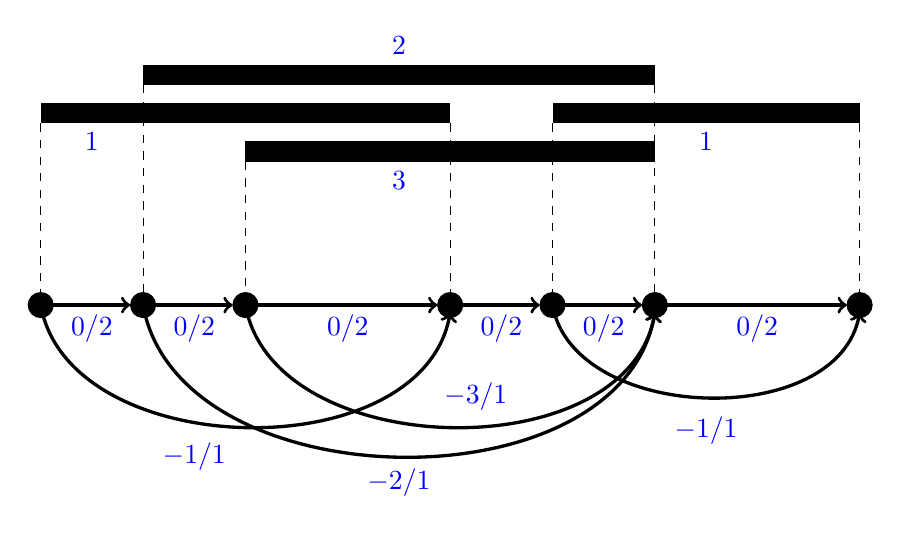
\begin{tikzpicture}[scale=0.65]

\fill (0,0.55) rectangle (8,0.95);
\draw (1, 0.55) node[below]{\textcolor{blue}{$1$}};

\fill (2,1.3) rectangle (12,1.7);
\draw (7, 1.7) node[above]{\textcolor{blue}{$2$}};

\fill (4,-0.2) rectangle (12,0.2);
\draw (7, -0.2) node[below]{\textcolor{blue}{$3$}};

\fill (10,0.55) rectangle (16,0.95);
\draw (13, 0.55) node[below]{\textcolor{blue}{$1$}};

      \foreach \x in {0,2,4,8,10,12,16}
        {\draw (\x,-3) node[fill,circle] {};}

        \draw[dashed] (0,0.55) -- (0,-3);
        \draw[dashed] (2,1.3) -- (2,-3);
        \draw[dashed] (4,-0.2) -- (4,-3);
        \draw[dashed] (8,0.55) -- (8,-3);
        \draw[dashed] (10,0.55) -- (10,-3);
        \draw[dashed] (12,1.3) -- (12,-3);
        \draw[dashed] (16,0.55) -- (16,-3);

        \draw[->,very thick] (0,-3) -- (1.75,-3);
        \draw (1, -3) node[below]{\textcolor{blue}{$0/2$}};
        \draw[->,very thick] (2,-3) -- (3.75,-3);
        \draw (3, -3) node[below]{\textcolor{blue}{$0/2$}};
        \draw[->,very thick] (4,-3) -- (7.75,-3);
        \draw (6, -3) node[below]{\textcolor{blue}{$0/2$}};
        \draw[->,very thick] (8,-3) -- (9.75,-3);
        \draw (9, -3) node[below]{\textcolor{blue}{$0/2$}};
        \draw[->,very thick] (10,-3) -- (11.75,-3);
        \draw (11, -3) node[below]{\textcolor{blue}{$0/2$}};
        \draw[->,very thick] (12,-3) -- (15.75,-3);
        \draw (14, -3) node[below]{\textcolor{blue}{$0/2$}};
        
        
        \draw[->,very thick] (0,-3) to[out=280, in=260] (8,-3.15);
        \draw (3,-5.5) node[below] {\textcolor{blue}{$-1/1$}};
        \draw[->,very thick] (2,-3) to[out=280, in=260] (12,-3.15);
        \draw (7,-6) node[below] {\textcolor{blue}{$-2/1$}};
        \draw[->,very thick] (4,-3) to[out=280, in=260] (12,-3.15);
        \draw (8.5,-5.25) node[above] {\textcolor{blue}{$-3/1$}};
        \draw[->,very thick] (10,-3) to[out=280, in=260] (16,-3.15);
        \draw (13,-5) node[below] {\textcolor{blue}{$-1/1$}};
\end{tikzpicture}
}

\only<3>{
\vspace{0.5cm}
Current flow = \textcolor{blue}{-2} $\Rightarrow$ Current weight =\textcolor{blue}{2}
\vspace{0.2cm}

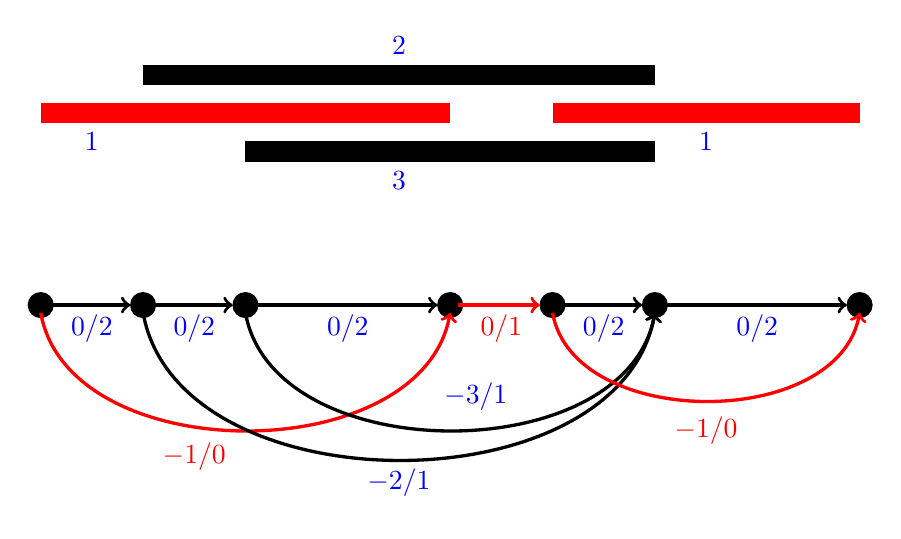
\begin{tikzpicture}[scale=0.65]

\fill[color=red] (0,0.55) rectangle (8,0.95);
\draw (1, 0.55) node[below]{\textcolor{blue}{$1$}};

\fill (2,1.3) rectangle (12,1.7);
\draw (7, 1.7) node[above]{\textcolor{blue}{$2$}};

\fill (4,-0.2) rectangle (12,0.2);
\draw (7, -0.2) node[below]{\textcolor{blue}{$3$}};

\fill[color=red] (10,0.55) rectangle (16,0.95);
\draw (13, 0.55) node[below]{\textcolor{blue}{$1$}};

      \foreach \x in {0,2,4,8,10,12,16}
        {\draw (\x,-3) node[fill,circle] {};}


        \draw[->,very thick] (0.15,-3) -- (1.75,-3);
        \draw (1, -3) node[below]{\textcolor{blue}{$0/2$}};
        \draw[->,very thick] (2.15,-3) -- (3.75,-3);
        \draw (3, -3) node[below]{\textcolor{blue}{$0/2$}};
        \draw[->,very thick] (4.15,-3) -- (7.75,-3);
        \draw (6, -3) node[below]{\textcolor{blue}{$0/2$}};
        \draw[->,very thick,color=red] (8.15,-3) -- (9.75,-3);
        \draw (9, -3) node[below]{\textcolor{red}{$0/1$}};
        \draw[->,very thick] (10.15,-3) -- (11.75,-3);
        \draw (11, -3) node[below]{\textcolor{blue}{$0/2$}};
        \draw[->,very thick] (12.15,-3) -- (15.75,-3);
        \draw (14, -3) node[below]{\textcolor{blue}{$0/2$}};
        
        
        \draw[->,very thick,color=red] (0,-3.15) to[out=280, in=260] (8,-3.15);
        \draw (3,-5.5) node[below] {\textcolor{red}{$-1/0$}};
        \draw[->,very thick] (2,-3.15) to[out=280, in=260] (12,-3.15);
        \draw (7,-6) node[below] {\textcolor{blue}{$-2/1$}};
        \draw[->,very thick] (4,-3.15) to[out=280, in=260] (12,-3.15);
        \draw (8.5,-5.25) node[above] {\textcolor{blue}{$-3/1$}};
        \draw[->,very thick,color=red] (10,-3.15) to[out=280, in=260] (16,-3.15);
        \draw (13,-5) node[below] {\textcolor{red}{$-1/0$}};
\end{tikzpicture}
}

\only<4>{
\vspace{0.5cm}
Total flow = \textcolor{blue}{-4} $\Rightarrow$ Total weight =\textcolor{blue}{4}
\vspace{0.2cm}

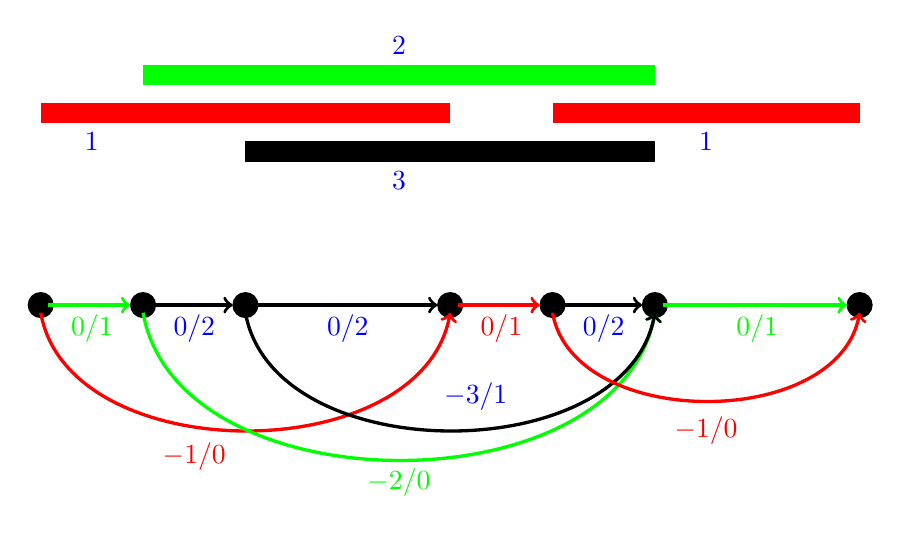
\begin{tikzpicture}[scale=0.65]

\fill[color=red] (0,0.55) rectangle (8,0.95);
\draw (1, 0.55) node[below]{\textcolor{blue}{$1$}};

\fill[color=green] (2,1.3) rectangle (12,1.7);
\draw (7, 1.7) node[above]{\textcolor{blue}{$2$}};

\fill (4,-0.2) rectangle (12,0.2);
\draw (7, -0.2) node[below]{\textcolor{blue}{$3$}};

\fill[color=red] (10,0.55) rectangle (16,0.95);
\draw (13, 0.55) node[below]{\textcolor{blue}{$1$}};

      \foreach \x in {0,2,4,8,10,12,16}
        {\draw (\x,-3) node[fill,circle] {};}


        \draw[->,very thick,color=green] (0.15,-3) -- (1.75,-3);
        \draw (1, -3) node[below]{\textcolor{green}{$0/1$}};
        \draw[->,very thick,] (2.15,-3) -- (3.75,-3);
        \draw (3, -3) node[below]{\textcolor{blue}{$0/2$}};
        \draw[->,very thick] (4.15,-3) -- (7.75,-3);
        \draw (6, -3) node[below]{\textcolor{blue}{$0/2$}};
        \draw[->,very thick,color=red] (8.15,-3) -- (9.75,-3);
        \draw (9, -3) node[below]{\textcolor{red}{$0/1$}};
        \draw[->,very thick] (10.15,-3) -- (11.75,-3);
        \draw (11, -3) node[below]{\textcolor{blue}{$0/2$}};
        \draw[->,very thick,green] (12.15,-3) -- (15.75,-3);
        \draw (14, -3) node[below]{\textcolor{green}{$0/1$}};
        
        
        \draw[->,very thick,color=red] (0,-3.15) to[out=280, in=260] (8,-3.15);
        \draw (3,-5.5) node[below] {\textcolor{red}{$-1/0$}};
        \draw[->,very thick,color=green] (2,-3.15) to[out=280, in=260] (12,-3.15);
        \draw (7,-6) node[below] {\textcolor{green}{$-2/0$}};
        \draw[->,very thick] (4,-3.15) to[out=280, in=260] (12,-3.15);
        \draw (8.5,-5.25) node[above] {\textcolor{blue}{$-3/1$}};
        \draw[->,very thick,color=red] (10,-3.15) to[out=280, in=260] (16,-3.15);
        \draw (13,-5) node[below] {\textcolor{red}{$-1/0$}};
\end{tikzpicture}
}

\end{overlayarea}

\end{frame}

\begin{frame}{Union/Find algorithm}

\begin{block}{Complexity in the case of preprocessed union tree}
\begin{itemize}
\item[$\bullet$] $\mathnormal{m}$: union and find intermixed operations
\item[$\bullet$] $\mathnormal{n}$: number of elements in the tree 
\end{itemize}
$\Rightarrow \mathnormal{O(m+n)}$ in time

\end{block}

\only<2>{
\begin{exampleblock}{Case of interval sets}
Union tree is a simple path.
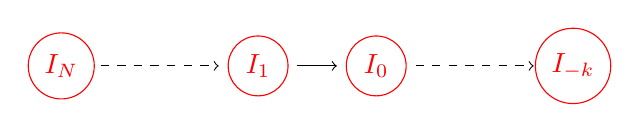
\begin{tikzpicture}
\node[draw, circle, red] at (0,0) {$I_{ N}$};
\draw[dashed,->] (0.5,0) -- (2,0);
\node[draw, circle, red] at (2.5,0) {$I_{ 1}$};
\draw[->] (3,0) -- (3.5,0);
\node[draw, circle, red] at (4,0) {$I_{ 0}$};
\draw[dashed,->] (4.5,0) -- (6,0);
\node[draw, circle, red] at (6.5,0) {$I_{-k}$};

\end{tikzpicture}
\end{exampleblock}

}

\only<3>{
\begin{exampleblock}{Case of interval sets}
Union tree is a simple path.
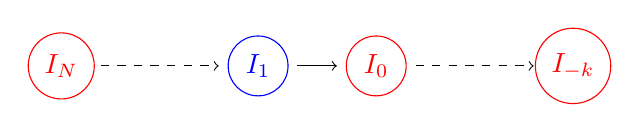
\begin{tikzpicture}
\node[draw, circle, red] at (0,0) {$I_{ N}$};
\draw[dashed,->] (0.5,0) -- (2,0);
\node[draw, circle, blue] at (2.5,0) {$I_{ 1}$};
\draw[->] (3,0) -- (3.5,0);
\node[draw, circle, red] at (4,0) {$I_{ 0}$};
\draw[dashed,->] (4.5,0) -- (6,0);
\node[draw, circle, red] at (6.5,0) {$I_{-k}$};

\end{tikzpicture}
\end{exampleblock}

}

\end{frame}

\section{Conclusion}

\begin{frame}{Applications}

\begin{block}{Register allocation}<1->
The goal is to minimize the number of variable load/store.\\ 
\textcolor{blue}{Variable use times} correspond to \textcolor{blue}{intervals}.\\
\textcolor{green}{Registers} correspond to \textcolor{green}{colors}.
\end{block}

\begin{block}{Job scheduling}<2->
You want to assign tasks to some identical \textcolor{green}{processors}. Each \textcolor{blue}{task} has a start time and an end time, plus a \textcolor{orange}{value}. The goal is to assign a set with the greatest task's value total.
\end{block}

\begin{block}{Wavelength assignment}<3->
The goal is to assign the maximum number of \textcolor{blue}{communication requests} to the different \textcolor{green}{wavelengths}.
\end{block}

\end{frame}


\begin{frame}{Conclusion}

\begin{block}{More about the article}
This article is twenty years old, but better algorithms do not exist\ldots
\end{block}

\begin{block}{Question}
Is it possible to have an even better complexity ?
\end{block}

\end{frame}

\plain{}{Questions}

\end{document}

